\documentclass[times,11pt]{report}
\usepackage{fullpage}
\usepackage{graphicx}
\usepackage[colorlinks=true,linkcolor=black]{hyperref}
\usepackage{hyperref}
\usepackage{mathptmx} % - sets \rmdefault to 'ptm', i.e. times
\renewcommand{\familydefault}{ptm} % using \rmdefault here doesn't work
\begin{document}
\title{Savant Genome Browser: User Manual}
%\author{Marc Fiume \& Eric Smith}
\maketitle

\setlength{\parindent}{0pt} 
\setlength{\parskip}{2ex}

Authors: Marc Fiume \& Eric Smith\\
Contact: savant@cs.toronto.edu \\
Website: http://savantbrowser.com \\
\\
This document applies to Savant version 2.0.0\\

\newpage

\tableofcontents
\listoftables
\listoffigures

\newpage

\chapter{Introduction}

\section{What is Savant?}

Savant stands for ``Sequence Annotation Visualisation and Analysis Tool''. In other words, Savant is a program for visualising and analysing genomics data. It was designed to run quickly and efficiently on conventional desktop or laptop computers.

\section{Who should use Savant?}

Savant makes visualisation and analysis of genomics data very efficient. If you use genome browsers like UCSC or IGV or if you are a biologist or bioinformatician who works with genomics data, you should try Savant. 

\section{Getting Started}
Savant is designed to run on any operating system which supports Java Standard Edition 1.6 or 1.7.  In practice, it has been tested on Windows (XP, Vista, and 7; 32-bit and 64-bit), Mac OSX (10.6 and 10.7), and Linux (32-bit and 64-bit).  An internet connection is strongly recommended.

When you launch Savant, you will be presented with the start screen, which shows a list of recent projects and a feed of news stories from the Savant web-site.  If this is the first time you have launched Savant, there will be no recent projects, so the first thing you should do is choose \textit{File~\textgreater~Load~Genome} to tell Savant what reference genome you wish to work with.

\chapter{Projects and Tracks}

When working with Savant you will typically be working with a number of ``tracks'' which are organised together into a ``project''.  In addition to the tracks, a project file also maintains associated information, such as the reference genome, your browsing location, and any saved bookmarks. Each track normally corresponds to single data file, although there are exceptions (e.g. a BAM alignment track may also be accompanied by a TDF file containing coverage information to be displayed at lower resolutions).  In order to be loaded as a track by Savant, a file must be in one of the formats described in Table~\ref{NativeFileFormats}.  Files which are not already in one of those formats can be converted as described in \S\ref{UsingFormatDialog}.

\section{Projects}
Projects have a file extension of .svp, and are typically stored in the .savant/projects directory.  The project stores the following information:
\begin{itemize}
\item Reference genome
\item Absolute paths of all loaded tracks.
\item Current display mode of all tracks
\item Bookmarks
\item For variant data, a summary of which participants are controls or cases (see Chapter~\ref{Variants})
\end{itemize}


\section{Genomes}
Before loading any tracks, the project's reference genome must be established using the \textit{File~\textgreater~Load~Genome} command.  This genome is used to specify the lengths and names of all chromosomes or contigs in the data set; no other tracks can be loaded until the genome has been set.  In many cases, the genome will itself be a sequence track, which can be loaded from a file, from a URL, or from a remote data-source.

For the convenience of users, a variety of standard published genomes are available from the Savant web-site.  The commonly-used genomes include a full sequence track along with associated tracks such as UCSC and RefSeq genes.  Less popular genomes may provide only a list of the chromosome names and their sizes.  The exact list is subject to change, and we welcome requests to add your favourite genomes to Savant's standard set.

In some unusual cases, you may wish to run Savant without any existing genome information.  In such cases, you can use the Load Genome dialog to specify a reference name and length.

\section{Tracks}

A track is an individual data set, usually corresponding to a single data file.  In a few situations a track may draw data from multiple data sources; this is the case for BAM alignment tracks which can have an associated TDF file containing coverage information to be displayed at lower resolutions.  In order to be loaded as a track by Savant, a file must be in one of the formats described in Table~\ref{NativeFileFormats}.  Files which are not already in one of those formats can be converted as described in \S\ref{UsingFormatDialog}.  If you attempt to load a track from one of the compatible file-types described in \S\ref{CompatibleFileFormats}, Savant will offer to format it first.

\subsection{Display Modes}
Every track type has one or more display modes.  Each of these modes is intended to emphasise a different aspect of the data. For instance, the \textit{Mismatch} mode for read alignment tracks, uses colours to emphasise mismatches in reads.  In contrast, the \textit{Read Pair (Arc)} mode emphasises the insert lengths, showing arcs between the mapped locations of paired reads, with the height of each arc proportional to the inferred insert size.  The display modes available for each type of track are described in \S\ref{TrackTypes}.

\subsection{Loading a Track}

A track is choosing one of the \textit{File~\textgreater~Load~Track} menu-items.  Track data can come from any of three different sources:  a local file, a URL, or an external data source.  \textit{Load Track from File} will present a file-chooser to let you select a local file.  \textit{Load Track from URL} presents a dialog which lets you type in an ftp://, http://, or https:// URL to be opened.

The \textit{Load Track from Other Datasource} menu-item presents the Savant repository browser, which lets you select one of the tracks which is available from savantbrowser.com.  In addition, this menu-item is also used by plugins such as the SQL and UCSC plugins to allow you to open a track using that plugin.

\subsection{Track Types}
\label{TrackTypes}

Savant supports five different types of tracks, which are described below.  Each track appears in a separate window, which can be manipulated as described in \S\ref{DockingFramework}.

At the right of the track is a legend which describes its contents.  Above the legend is a track-specific menu-bar which allows you to control the display and behaviour of that track.  This menu-bar will have at least two items:  Tools and Appearance.  In addition, some tracks have menu items which let you control \textit{Display Mode} and \textit{Interval Height}.

The \textit{Tools} menu provides useful functionality such as the ability to Lock a track (see \S\ref{TrackLocking}) and to copy the track's URL to the clipboard.  Track types which have the ability to filter their contents add a Filter� item to the Tools menu, which invokes a dialog to specify filter parameters.

The Appearance menu controls the track's colour settings.  For tracks which have a vertical scale (all but sequence tracks), the \textit{Scale to Fit} menu-item controls whether the track scales its y-axis to fit the size of the window or uses a vertical scrollbar when necessary.

\subsubsection{Sequence Tracks}
Sequence tracks take their data from a .fa or .fa.savant\footnote{.fa.savant files store sequence data in a format specific to Savant versions prior to 2.0.0.} file.  They display a sequence of colour-coded nucleotides.

Sequence tracks are often used by \textit{File~\textgreater~Load~Genome} to provide the reference genome for a project.  If you have more than one sequence track open in a project, you can use a sequence track's \textit{Tools~\textgreater~Set~as~Genome} menu-item to make it the reference genome.

\subsubsection{Interval Tracks}
Interval tracks display data from a Tabix file.  This is the track-type for genes and other interval-oriented data.

Interval tracks have two display modes:  Standard and Squish.  In Standard mode intervals are packed neatly so that none overlap; in Squish mode, the intervals are squished together on a single line.  These correspond to the Pack and Squish modes of the UCSC browser. 

In addition, interval tracks also have a number of Appearance options.  The \textit{Enable ItemRGB} option colours records based on the value of their ItemRGB column (for BED files which have that column).  Similarly, for BED files with a Score column, the \textit{Enable Score} option allows you to draw records with a transparency based on the Score value. The \textit{Display Alternate Name} option allows you to control which labels are displayed for the features (e.g. for gene tracks which may identify genes with both accession numbers and protein IDs).

\subsubsection{Alignment Tracks}

Alignment tracks display data from a BAM file.  They present reads in a choice of seven different display modes, listed in Table~\ref{AlignmentModes}.

\begin{table}[h]
\label{AlignmentModes}
\begin{center}
\begin{tabular}{|l p{5in}|}
\hline
Standard & Displays the reads stacked vertically in the most efficient manner.  Colour indicates strand direction.\\
Mismatch & Like Standard, but also displays SNPs and indels.  Requires that the reference genome be an actual sequence track.\\
Read Sequence & Displays the reads stacked vertically, but colour indicates nucleotides.\\
Read Pair (Standard) & Reads are stacked vertically, with paired reads are at the same altitude.\\
Read Pair (Arc) & Read pairs are shown using arcs, where the height of the arc corresponds to the inferred insert size.\\
SNP & For each location, all the base-reads supporting a particular call are stacked vertically.  This is intended to make SNPs more prominent.\\
Strand SNP & Like SNP mode, but reads from the forward and reverse strands are grouped separately.\\
\hline
\end{tabular}
\end{center}
\caption{Alignment Track Display Modes}
\end{table}

In addition to the display mode, you can also adjust the appearance of the Standard, Mismatch, and Read Sequence modes by using the \textit{Enable Base Quality} and \textit{Enable Mapping Quality} items from the \textit{Appearance} menu.

When the visible range is large enough that individual reads would not be visible, Savant will display a coverage graph (\S{GeneratingCoverageFiles}) in place of the normal display.

\subsubsection{Continuous Tracks}
Continuous tracks display continuous-valued data from TDF or BigWig files.

\subsubsection{Variant Tracks}
Variant tracks display structural variation data from Tabix-formatted VCF files.  The vertical axis is used to indicate the individuals whose data makes up the file.  Data from all loaded variant tracks is aggregated in the Variation sheet described in \S\ref{Variants}.

\chapter{Formatting and Loading Data}

\section{Supported File Formats}

Savant natively supports a number of standard file formats which are indexed to ensure speedy data retrieval.  In addition, Savant has the ability to reformat several other common formats in order to make them usable by the program.

\subsection{Native File Formats}

Savant natively supports the following standard file formats.  These are formats which Savant can read directly with no extra processing.  In most cases, these files consist of a main file which contains the actual data and an index file which is must be present in the same location as the data file in order to provide fast random access to that data.

\begin{table}[ht] 
\begin{center}
\begin{tabular}{|l|l|l|l|}  
\hline                      
Format & Description & Data File & Index File\\
\hline                    
\href{http://genome.ucsc.edu/goldenPath/help/bam.html}{BAM} & Nucleotide  sequence alignments & .fa & .fai \\
\href{http://genome.ucsc.edu/goldenPath/help/bigWig.html}{BigWig} & Continuous-valued data & .bw & \\
\href{http://genetics.bwh.harvard.edu/pph/FASTA.html}{FASTA} & Nucleotide sequences & .fa & .fai \\
\href{http://samtools.sourceforge.net/tabix.shtml}{Tabix} & Genes, intervals, variants, and other localised data & .gz & .tbi \\
\href{http://www.broadinstitute.org/igv/TDF}{TDF} & Any continuous-valued data & .tdf & \\
\hline     
\end{tabular} 
\caption{Native File Formats}
\label{NativeFileFormats}
\end{center}
\end{table} 

\subsection{Compatible File Formats}
\label{CompatibleFileFormats}

These are formats which Savant can convert into one of its native formats.  When using a file in one of these formats, it must first be converted into one of Savant�s native formats.
You can convert these files either by using choosing Format from Savant�s File menu, or by using Savant�s \textit{FormatTool} utility.

\begin{table}[ht] 
\label{CompatibleFileFormatsTable}
\begin{center}
\begin{tabular}{|l|p{3in}|l|}  
\hline                      
Format & Description & Converted To\\
\hline                    
\href{http://genome.ucsc.edu/FAQ/FAQformat.html#format1}{Bed} & genes, intervals, variants, and other localised data & .tabix \\
\href{http://genome.ucsc.edu/goldenPath/help/bedgraph.html}{BedGraph} & continuous-valued data & .tdf \\
\href{http://www.sanger.ac.uk/resources/software/gff/spec.html}{GFF/GTF} & genes and other features associated with DNA, RNA and protein sequences & .tabix \\
Tab-delimited & any feature-oriented data in tab-delimited form & .tabix \\
\href{http://www.1000genomes.org/node/101}{VCF} & structural variations & .tabix \\
\href{http://genome.ucsc.edu/goldenPath/help/wiggle.html}{Wig} & continuous-valued data such as GC percent, probability scores, and transcriptome data & .tdf \\
\hline
\end{tabular}
\caption{Compatible File Formats}  
\end{center} 
\end{table} 

\begin{minipage}{6.5in}
Genomic annotations are also available from other databases. Downloading and formatting data from these and other popular data sources is encouraged:\\

\begin{tabular}{l l}
UCSC & \href{http://genome.ucsc.edu}{http://genome.ucsc.edu}\\
1000 Genomes Project & \href{http://www.1000genomes.org}{http://www.1000genomes.org}\\
NCBI & \href{http://www.ncbi.nlm.nih.gov}{http://www.ncbi.nlm.nih.gov}\\
EBI & \href{http://www.ebi.ac.uk}{http://www.ebi.ac.uk}\\
\end{tabular}
\end{minipage}

\section{Using the Format Dialog}
\label{UsingFormatDialog}

The Format Dialog can be used to format text files (e.g. ones downloaded from the various data sources listed above) for use with Savant. In most cases, Savant is able to infer the file's format from its extension.  Given the size of data files associated with bioinformatics, formatting a file may take a considerable amount of time.

The Format Dialog can be opened by choosing File~\textgreater~Format File. \\

\begin{figure}
\label{FormatDialog}
\begin{center}
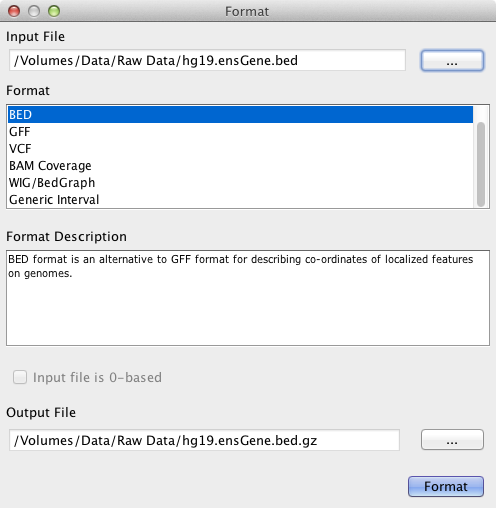
\includegraphics[type=png,ext=.png,read=.png,height=8cm]{images/FormatDialog}
\caption{The Format Dialog}
\end{center}
\end{figure}

Components of the Format Dialog (Figure \ref{FormatDialog}):
\begin{description}
\item[Input file]The text file to be formatted
\item[Format]The format of the input file
\item[Input is 1-based]Whether or not the input file's positional annotations start at 0 or 1.  In most cases, this is determined by the choice of Format.
\item[Output file]The output file to be produced which can subsequently be loaded into Savant
\end{description}

\subsection{Generating Coverage Files}
\label{GeneratingCoverageFiles}
In addition to formatting the file types described in Table~\ref{CompatibleFileFormatsTable}, the Format dialog is also used for generating coverage files.  These are used to display alignment data when the viewable range is too large to make individual reads discernible.  In such cases, Savant uses the coverage file to draw a continuous track indicating the level of read coverage across the viewable range.  Simply choose a .bam file as the input, and Savant will generate the corresponding .bam.cov.tdf file.  In order to serve as a coverage file, the .bam.cov.tdf file must be stored in the same location as the .bam file which it summarises.


\chapter{Navigation}

Navigation refers to changing the region of the genome which is viewed by the browser. A user can navigate by either interacting with the navigation toolbar (\S\ref{NavigationToolbar}) located at the top of the Savant main window, or by using the appropriate keyboard and mouse shortcuts (\S\ref{NavigationShortcuts}).

In Savant a location consists of two parts:  the current reference and the current visible range.  The current reference is typically a chromosome, so the terms ``chromosome'' is used below, even though the reference in question could actually be any contiguous range of bases, and not necessarily a chromosome \textit{per se.}

\section{Navigation Toolbar}

\begin{figure}[h]
\label{NavigationToolbar}
\begin{center}
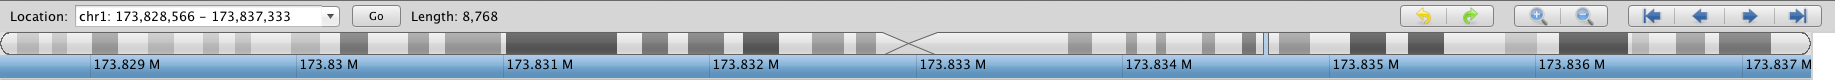
\includegraphics[type=png,ext=.png,read=.png,width=7in]{images/NavigationBars}
\caption{Navigation Toolbar}
\end{center}
\end{figure}

The top row of the navigation toolbar contains the location field (\S\ref{LocationField}) and the navigation buttons (\S\ref{NavigationButtons}).  Below that are the range selection bar and the ruler (\S\ref{RangeSelectionBar}).

\subsection{Location Field}
\label{LocationField}
\begin{figure}[h]
\begin{center}

\includegraphics[type=png,ext=.png,read=.png]{images/LocationField}
\caption{Location Field}
\end{center}
\end{figure}

The location field displays the current visible range within the genome.  It can also be used to specify a new range in a number of ways, described in the table below.  Changes take effect by hitting {\sc return} or clicking the \textit{Go} button.

\begin{table}[h]
\begin{center}
\begin{tabular}{|l l l|}
\hline
1) & \multicolumn{2}{l|}{Clicking the downward-pointing triangle to reveal a menu of chromosomes.}\\
\hline
2) & \multicolumn{2}{p{6in}|}{Type a gene name into the text field or type a partial gene name and hit {\sc tab} to pop up a menu of matching genes.}\\
\hline
3) & \multicolumn{2}{l|}{Type a range specification into the text field:}\\
& &\\
& chr2:1000-2000 & chr2, range 1000-2000\\
& chr2: & the current range, but in chr2\\
& 1000-2000 & in current chromosome, range 1000-2000\\
& 1000-900 & in current chromosome, range 900-1000 (equivalent to 900-1000)\\
& 1000+2000 & in current chromosome, range 1000-3000\\
& 1000 & in current chromosome, start position at 1000, keeping current range-length\\
& +1000 & 1000 bases to the right of the current start, keeping same range-length\\
& -1000 & 1000 bases to the left of the current range, keeping same range-length\\
\hline
\end{tabular}
\caption{Specifying Ranges Using the Location Field}
\end{center}
\end{table}

\subsection{Navigation Buttons}
\label{NavigationButtons}

\begin{figure}[h]
\begin{center}

\includegraphics[type=png,ext=.png,read=.png]{images/NavigationButtons}
\caption{Navigation Buttons}
\end{center}
\end{figure}
At the top right of the Navigation Toolbar are eight buttons which perform a variety of navigation-related tasks.  From left to right these are:  \textit{Undo, Redo, Zoom In, Zoom Out, Beginning, Pan Left, Pan Right,} and \textit{End.}

\textit{Undo} lets you undo your previous navigation action.  It can be used repeatedly to undo multiple navigation actions.  \textit{Redo} cancels the effect of the most recent \textit{Undo.}

\textit{Zoom In} and \textit{Zoom Out} change the visible range by a factor of two, keeping it centred on the same location.

\textit{Pan Left} and \textit{Pan Right} shift the visible location left or right by half the width of the screen.

\textit{Beginning} and \textit{End} allow you to navigate quickly to the beginning or end of the current chromosome.

\subsection{Range Selection Bar and Ruler}
\label{RangeSelectionBar}

\begin{figure}[h]
\begin{center}
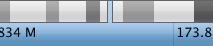
\includegraphics[type=png,ext=.png,read=.png]{images/RangeSelection}
\caption{Range Selection Bar and Ruler}
\end{center}
\end{figure}
Below the location field and the navigation buttons lies the range selection bar.  This bar highlights in blue the current visible region in the context of the genome. If the current genome has associated cytoband information, it will be displayed in this bar.  Users can select a new range by clicking and dragging within the bar.

Underneath the range selection bar is the ruler, which indicates the current viewable range in the coordinate space of the current chromosome.

\section{Mouse and Keyboard Shortcuts}
\label{NavigationShortcuts}
Navigation can be done very quickly using a number of mouse and keyboard shortcuts described in the tables below.

\begin{table}[ht] 
\begin{center}
\begin{tabular}{|l l|}
\hline
Keys & Action \\
\hline                    
{\sc shift}+{\sc left} & pan left  \\
{\sc shift}+{\sc right} & pan right \\ 
{\sc shift}+{\sc home} & move to start of chromosome  \\
{\sc shift}+{\sc end} & move to end of chromosome \\ 
{\sc shift}+{\sc up} & zoom in \\
{\sc shift}+{\sc down} & zoom out \\  
\hline
\end{tabular}
\caption{Navigation Using the Keyboard}  
\end{center}
\end{table} 

\begin{table}[ht] 
\begin{center}
\begin{tabular}{|l l|}  
\hline                      
Keys & Action \\
\hline            
Click and drag left/right & pan left/right  \\
{\sc ctrl/cmd} + scroll-wheel up/down & pan left/right  \\
{\sc ctrl/cmd} + Click and drag & zoom in on selected region  \\
{\sc shift} + Click and drag  & select all records in region  \\
\hline     
\end{tabular}
\caption{Navigation Using the Mouse}  
\end{center}
\end{table} 

\section{Other Useful Shortcuts}

Range changes can be undone and redone using the commands in the following table. 

\begin{table}[h] 
\begin{center}
\begin{tabular}{|l l|}  
\hline                      
Keys & Action \\
\hline                    
{\sc ctrl/cmd}+{\sc z} & undo range change  \\
{\sc ctrl/cmd} + {\sc y} & redo range change \\ 
{\sc ctrl/cmd} + {\sc i} & export track images (see \S\ref{ExportingImages}) \\ 
{\sc ctrl/cmd} + {\sc b} & bookmark current location (see \S\ref{Bookmarks}) \\ 
\hline
\end{tabular}
\caption{Other Shortcuts}  
\end{center}
\end{table} 

\chapter{Docking Framework}
\label{DockingFramework}

Savant features a docking framework which allows users to rearrange modules to their liking. Such modules include tracks and built-in items (e.g. Bookmarks, Variants, etc.) and plugins. Non-track modules are constrained to be docked to the sides of the UI and not among tracks. Similarly, track modules are constrained so that they cannot be docked among other modules.

While a number of important functions are presented here, the best way to learn all the features of the docking framework is to try using it.

\begin{figure}
\begin{center}
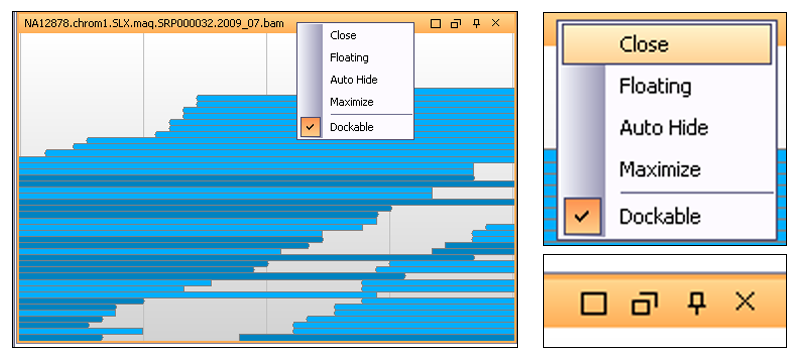
\includegraphics[type=png,ext=.png,read=.png,width=12cm]{images/dockingcontrols}
\caption{Left: A track module. Upper-right: Docking menu presented when the title bar of a module is right-clicked. Bottom-right: Docking controls embedded in the title bar of the module. The latter controls are {\it not} available in the Mac version.}
\end{center}
\end{figure}

\section{Showing and Hiding Modules}

By default, built-in modules are hidden. Hidden modules appear as tabs located on the region of the UI to which they are docked. A module is shown once the tab is clicked. Click the tab again to hide the module.

\begin{figure}
\begin{center}
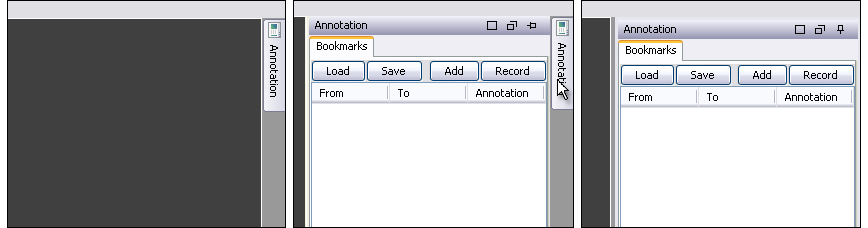
\includegraphics[type=png,ext=.png,read=.png,width=14cm]{images/hideshowmodules}
\caption{Hiding and showing modules. Left: The Annotation module, hidden on the right of the Savant UI. Middle: The Annotation module, shown by mousing over the Annotation tab. Right: The Annotation module, pinned so that it will remain shown even when the user is interacting with other components of the UI. }
\label{HideShowModules}
\end{center}
\end{figure}

\section{Resizing Modules}

Modules can be resized. To resize a module, click an edge and drag it until it occupies the desired size. 

\section{Rearranging modules}

Modules can be arranged in virtually any configuration within the UI. To move a module, click its title bar and drag it to the desired new location. While dragging, a grey outline will appear showing the location the module will occupy if the mouse is released. Track modules can be docked to the top or bottom of the track space, while other modules can be docked to any edge of the UI. In addition, modules can be docked on top of each other (in which case tabs will appear allowing one to switch between modules) or beside each other.

\begin{figure}
\begin{center}
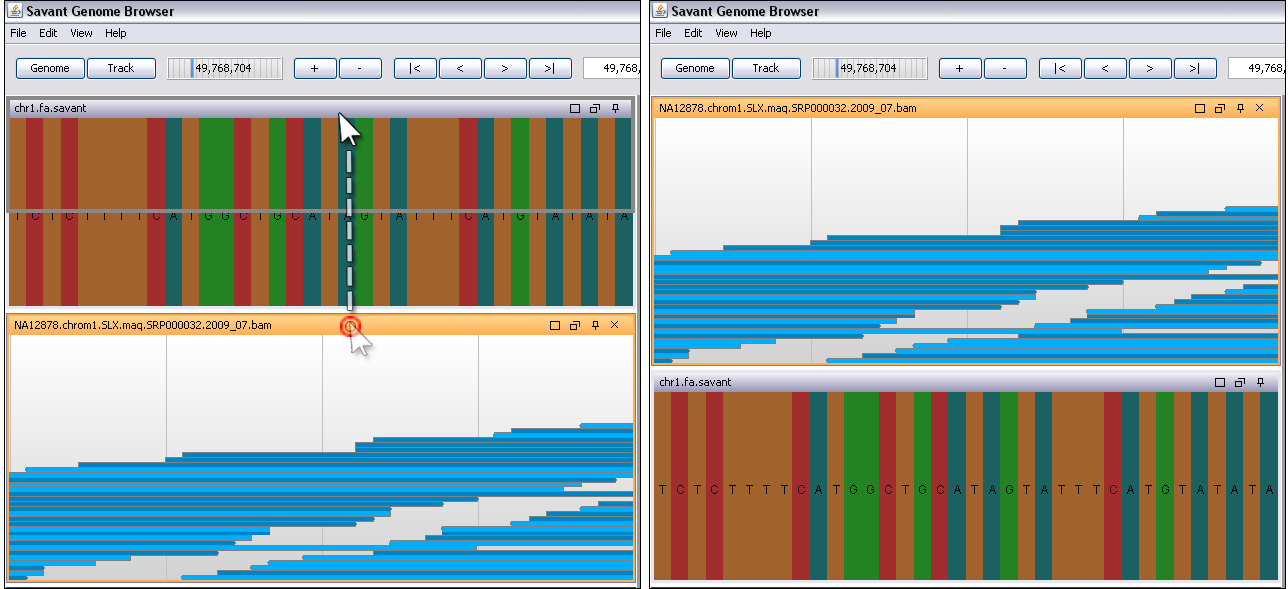
\includegraphics[type=png,ext=.png,read=.png,width=14cm]{images/arrangemodules}
\caption{Rearranging modules. Left: Demonstration of the rearrangement process. Right: The result of the rearrangement.  }
\label{ArrangeModules}
\end{center}
\end{figure}

\section{Maximising and Restoring Modules}

A module can be maximised to occupy the entire screen or UI, to make interaction or visualisation with it easier, and then restored back to its original state among other modules to resume a concerted view. To maximise, press the embedded icon which resembles a square. To restore, press the embedded icon which resembles two overlapping squares (in the same location as the icon pressed to maximise). On a Mac, you can maximise and restore by right-clicking the title bar and click maximise and restore, respectively. The same functionality is possible through the title bar on Windows and Linux.

\section{Detaching and Attaching from and to the UI}

A module can be detached from the UI and moved to a separate location on the screen. This is particularly useful for multidisplay setups where, for example, analytics modules can be moved to one display and tracks kept on another. To detach a module, press the embedded icon which resembles to squares. The detached module can then be moved to another location by clicking and dragging its title bar. To reattach it to the UI, press the embedded icon which resembles a square with an L-shape in it (in the same location as the icon pressed to detach it). On a Mac, you can detach and reattach by right-clicking the title bar and checking or unchecking Floating, respectively. The same functionality is possible through the title bar on Windows and Linux.


\chapter{Bookmarks}

The Bookmarks module helps to keep track of interesting regions or to make annotations. At any time, users may add, remove, or seek to a bookmarked region by using buttons within the module or by using keyboard shortcuts. 

\begin{figure}
\begin{center}
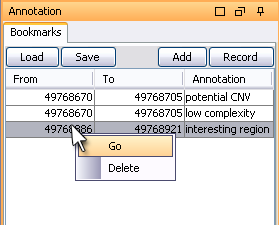
\includegraphics[type=png,ext=.png,read=.png,width=6cm]{images/bookmarks}
\caption{Bookmarks Module}
\label{BookmarksModule}
\end{center}
\end{figure}

\section{Adding and Removing Bookmarks}

A bookmark can be added by pressing the Add button embedded in the Bookmarks module. The current range will be used for the bookmark, although the from and to coordinates of the bookmark can be adjusted by double clicking and changing them. The keyboard shortcut CTRL+B (or CMD+B on a Mac) can be used to quickly add a bookmark. Bookmarks can be removed by right clicking them and choosing the Delete option.

\section{Seeking to a Bookmark}

A bookmark can be sought to by right clicking it and choosing the Go option.

\section{Adding annotations to bookmarks}

An annotation can be added to a bookmark by double-clicking the Annotation field and typing in some text. 

\section{Recording Navigation History}

Navigation history can be tracked by clicking the Record button embedded in the Bookmarks module. From then on, every new range viewed will be stored as a Bookmark. To stop recording, press the Stop Recording button.

\section{Saving and loading bookmarks}

Bookmarks can be saved, to be reused in future sessions or to be shared with colleagues. To save the existing bookmarks, click the Save button embedded in the module. These bookmarks can subsequently be loaded by clicking the Load button embedded in the module. A user can opt to append the loaded bookmarks to the existing bookmarks, or to replace the existing bookmarks entirely with the loaded ones.

\chapter{Table View}

The Table View module displays the data in the current range in a tabular format. This module displays records as rows and fields as columns
in a spreadsheet. The data is automatically updated when a range is changed, unless the Auto Update checkbox is unchecked.

\begin{figure}
\begin{center}
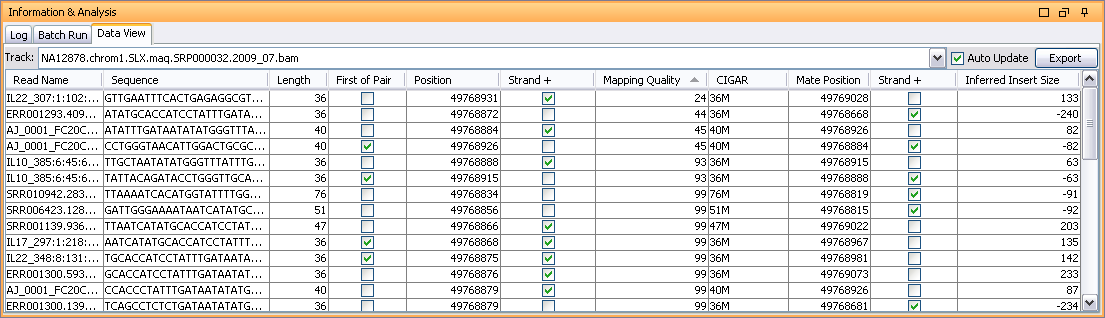
\includegraphics[type=png,ext=.png,read=.png,width=16cm]{images/tableview}
\caption{Table View module, showing data from a read alignment track.}
\label{TableView}
\end{center}
\end{figure}

\section{Changing tracks}

The Table View only displays data from a single track at a time. To change the track whose data is being displayed, a drop-down list of tracks is provided from which to chose from.

\section{Sorting rows}

The entries in the Table View can be sorted by clicking the field header by which the rows are to be sorted.

\section{Exporting Data}

The data in the Table View can be exported by clicking the Export button embedded in the module. The resulting file is a tab-delimited encoding of the information shown in the browser.

\chapter{Plugins}

Savant is able to integrate plugins, allowing for powerful extensions of the browser. To learn how to develop a plugin, see the {\bf Developer's Guide} downloadable from the Savant website.

\section{Installing a plugin}

To install a third-party plugin, copy the plugin's .jar file to the Savant/plugins directory and restart Savant.

\section{Un-installing a plugin}

To un-install a third-party plugin, remove the plugin's .jar file from the Savant/plugins directory and restart Savant. Do not remove the SavantCore.jar file at any time.

\section{Using a plugin}

Every plugin works differently and may or may not have a user interface. For instructions on how to use a third-party plugin, see the developer's documentation.

\chapter{Other Features}

\section{Track Locking}
\label{TrackLocking}
Individual tracks can also be locked to a particular range so that they are not updated until they are unlocked. Locked tracks can be used as overview profiles from which subregions can be selected to specify range changes for other tracks. To lock a track, right-click inside the track module and check the Lock option. While a track is locked, users may select a subrange from the track (by using the mouse zoom options, described previously) which will become the new range for other, unlocked tracks. To unlock a track, right-click inside the track module and uncheck the Lock option.

\section{Selecting}
In most cases, a track consists of a selection of underlying records, which can be selected individually.  By default, selected records are highlighted in green.
\section{Exporting Images}
\label{ExportingImages}

\chapter{Variants}
\label{Variants}

\end{document}
